In this section we present a framework to collect and analyze data needed for performance diagnosis from the point of view of a virtual guest system. 
First, we define the layers of abstraction and virtual resources unique to virtual environments.  
Then we identify the additional information needed from these layers, and a method to collect the data.
Finally, we describe a method to analyze the additional data to determine if the guest machine is experiencing external I/O interference.

In order to accurately determine if interference is due to external interference, we need to first calculate the overhead and establish a known baseline for that configuration.  Then, when run in production with other systems, we can compare the latency and throughput at the guest and hypervisor layers.  

% 1 Define the new layers of abstraction virtual environments.
\subsection{Abstraction Layers and Resources}
On a single physical server, the application, OS, and hardware layers need to be considered as a potential problem for application performance problems.  The resources are physical hardware such as a disk, memory (RAM), and the CPU cores (Figure \ref{PhysicalLayers}).  Applications access the physical resources through the kernel, and the kernel tracks statistics about the usage of the resource.  The availability of the physical resource is known or meets some sort of guarantee from the hardware.

\begin{figure}[!h]
  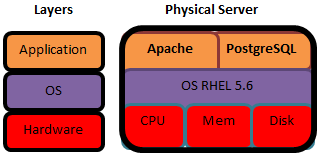
\includegraphics[width=3in]{images/LayersPhysical.png}
  \caption{Layers in physical server.  OS kernel tracks statistics about physical hardware.}
  \label{PhysicalLayers}
\end{figure}

In a virtual environment, the OS layer in the guest virtual machine does not have direct access to the physical resources.  Instead the hypervisor divides the physical resources between the guest systems and presents a virtual resource to the guest OS (Figure \ref{LayersAndResources}).
This is similar to an OS kernel dividing up the CPU time between multiple processes, where each process only runs for a portion of the total CPU time.  
The major difference between an OS kernel dividing up a physical resources, and the hypervisor dividing up a resources is that the OS layer provides APIs to the application layer in order to monitor the resources.  By default (on Linux and Windows) any process can determine the percentage of resources that it is using.  Unlike the OS kernel layer, the hypervisor layer provides little or no information to the layer above it about the true availability and use of the resource. 

\begin{figure}[!h]
  \begin{center}
  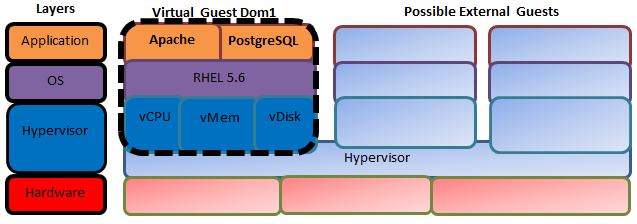
\includegraphics[width=6in]{images/LayersVirtual.png}
  \caption{New layer \textbf{Hypervisor} should share information with guest OS about physical resources.  The guest OS kernel now tracks statistics about the virtual resources.}
  \label{LayersAndResources}
  \end{center}
\end{figure}

The physical resource may be used by an external virtual machine or by the hypervisor, and there is little information that a guest OS or application can see about the availability of the physical resource.
Additionally, the hypervisor view does not know about specific processes running in the guest.  If the VMM performance tools could identify the resource availability, there is not any way to relate that to a specific guest process.  Both the virtual guest administrator and hypervisor administrator would need to monitor resources concurrently and share infomration through an external channel. 
Additional information is needed immediately from hypervisor about the physical resource so that the administrator, OS, or application can make better decisions about the availability of the resource. 

\begin{table}[h]
  \begin{tabular}{ l p{10cm} }
    Resource & Definition \\
    \hline
    vCPU & The virtual core allocated to the guest \\
    vMemory & The virtual RAM allocated to the guest \\
    vDisk I/O & The virtual I/O block device allocated to the guest \\
    \hline
  \end{tabular}
\caption{Virtual resources which may experience interference from hypervisor or external guest.}
\label{tab:resources}
\end{table}

% 3 Identify the performance counters which can be used to measure I/O performance on a virtual guest machine.
\subsection{Performance statistics}
To monitor applications and the kernel, administration tools will read kernel statistics over some period of time.  Then the tool will aggregate and relate the data for that time period.  In some cases, additional inference can be made from different parts of the data.  For example the \emph{sar} utility can show the average wait time, average service time, and bandwidth utilization for I/O.  On a physical server, where the hardware availability is deterministic, this information is valuable for analyzing and tuning applications.  However, when the resource is virtualized, these kernel resource statistics for virtual resources are almost meaningless, because the availability of the physical resource is not known.  Our tests will show that for disk I/O statistics, there is little difference in these counters when comparing application load changes and interference from external virtual guests. 

\begin{figure}[h]
\begin{algorithmic}[H]
 \STATE $interval \gets 5$
 \STATE $stat \gets$  DiskRead       
 \STATE $pre \gets $ READ $stat$ 
 \LOOP
    \STATE SLEEP $interval$
    \STATE $post \gets$ READ $stat$
    \STATE $result \gets (post - pre)/interval$
    \STATE PRINT  $result$
    \STATE $pre \gets post$ 
 \ENDLOOP
\end{algorithmic}
\caption{Example to display reads per second \emph{reads/s} every 5 seconds.}
\label{alg1}
\end{figure}

Our method will collect, aggregate, and analyze the statistics kept by the guest OS and hypervisor layers in order to measure interference from external domains and the hypervisor.  We find that there are statistics that will show the interference from external machines, when collected from all layers.  For our examples we choose disk read and virtual memory statistics to analyze I/O read bottlenecks.  However, this method could be used for identifying other types of performance problems if the data was available to the guest.

\begin{table}[h]
\begin{subtable}[h]{0.45\textwidth}
\caption{Virtual memory paging performance counters \cite{memory}}
\begin{tabular}{ l l }
       pgpgin  &  count of memory pages in. \\
       pgpgout  & count of memory pages out. \\
       pgfault  & count minor (or soft) page faults. \\
\end{tabular}
\label{fig:memory}
\end{subtable}
\hfill
\begin{subtable}[h]{0.45\textwidth}
\caption{I/O read performance counters \cite{iostats}}
\begin{tabular}{ l l }
       r\_sectors & number of sectors read successfully. \\
       r\_ms & number of milliseconds spent by all reads. \\
       r\_total & number of reads completed successfully. \\
\end{tabular}
\label{fig:io}
\end{subtable}
\caption{Statistics collected from all guests and hypervisor}
\end{table}

By collecting these statistics at two points in time as in Figure \ref{alg1}, we can infer other data such as the throughput in reads per second \emph{reads/s}.  We can also calculate the average wait time for reads \emph{AvgRdWait}.  
Since \emph{r\_ms} is the total number of milliseconds spent by all reads, we can divide this by the total number of reads to get the average wait time.  This is very important since external guests may cause I/O delays for a shared disk accessed concurrently by multiple guests.
\newline\newline
\Large
	$AvgRdWait = \frac{r\_ms}{r\_total}$   Average Read Wait Time\\
	$reads/s = \frac{r\_total}{TotalTime}$  Average Read Throughput \\
\normalsize

% 4 A method to calculate the overhead and theoretical maximum performance using an off-line modeling technique.
\subsection{I/O Virtualization Overhead}
For each virtual resource (Table \ref{tab:resources}) there is a performance cost to making that resource virtualized.  If the guest had direct access to the hardware, at all times, the virtualization cost would be zero.  Since most system calls from the guest kernel need to go through the hypervisor, we need to account for this additional time.

Several researchers \cite{cherkasova, huber1} have called this cost the \emph{overhead}, and have quantified the overhead for a given configuration.  This previous research used an off-line modeling technique by running a benchmark with and without virtualization.  By calculating the percent difference of these two benchmarks they can calculate the overhead.
The problem with this technique is that physical servers would need to be provisioned for this exercise.  Any configuration changes in hardware or anywhere in the software stack, may require a new test.  

Our method uses a similar approach, but does not require physical hardware for each guest.  We calculate the percent difference between the counters for the physical resources in the hypervisor and the virtual resources in the guest. 
We claim that the time spent waiting for an operation to complete in one layer depends on the layer below.  
In a physical server the application depends on the kernel and the kernel depends on the hardware.  
Our overhead calculation finds this additional time for I/O virtualization, by using the $AvgRdWait$ statistic in both the guest and hypervisor without interference to calculate the overhead.

We need to calculate the \emph{overhead} before running a guest virtual machine in production. 
In data centers and cloud systems, templates are usually created before virtual machines are used in production.  A template is a complete snapshot image of a virtual machine that has been built and tested to meet some need.  For example a Redhat 6.2 system with an Apache web server may need to be used on several machines.  A system could be built, tuned, and tested for that environment and then made into a template.  Future users can deploy a new virtual machine from that template.  We suggest to calculate the overhead from virtualization before it is made into a template.  

To calculate the virtualization overhead, create a single virtual machine with dedicated resources on isolated hardware.  
There are many performance benchmarks that can be used \cite{katcher, tikotekar, hplBench} to place a desired load on the virtual machine. 
Then run the benchmark or load on the virtual machine and begin monitoring the performance statistics for that resource using the algorithm in Figure \ref{alg1} in both the guest OS and hypervisor. 
Save the results of the guest, hypervisor, and time in the guest as this is the baseline statistic without external interference.
It is important that the guest and hypervisor collect \emph{pre} and \emph{post} statistics as close to the same time as possible.  

Since we are measuring from the perspective of the guest OS, we want to discover how the guest degrades in comparison to the hypervisor.  
For some statistics such as the \emph{AvgRdWait}, we can approximate the overhead of virtualization, by calculating the average wait time in the hypervisor \emph{AvgRdWait\textsubscript{H}} and the guest \emph{AvgRdWait\textsubscript{G}}.

\begin{equation}
  Overhead_{IO} = \frac{AgvRdWait_G - AvgRdWait_H}{AvgRdWait_H} 
\end{equation}

% Simple method %
\subsection{I/O Virtualization Interference}
We should be able to distinguish between a guest that is degraded because the hypervisor layer (including external interference) is using the resource and a guest that is degraded because of an application or OS layer issue within the guest.  In other words we should be able to distinguish between a problem inside the guest and a problem where the guest has no control.  An secondary goal is to measure or analyze the interference.  We should be able to answer the question, "How much of the resource is available to the guest?".

It may seem possible to that we can determine degradation by examining only the resource statistics inside of the guest machine.  However, with some simple tests, we were able to change the I/O wait and throughput in a guest domain by only changing the guest workload and data size (Table \ref{tab:guestOnly}).
 
% See barbaro_Dom29.txt %
\begin{table}[h]
  \begin{tabular}{ l l p{5cm} }
    Test & $AvgRdWait$ & $reads/s$  \\
    \hline
    Baseline                     & 5.96 & 376 \\   % Test 1
    Increase DB size             & 8.04 & 563 \\   % Test 3
    Increase DB Connections      & 20.3 & 875 \\   % Test 4
    Decrease DB Connections      & 4.94 & 144 \\   % Test 5
    Baseline with Interference   & 9.86 & 242 \\   % Barbaro Exp7.2 (P2)
    \hline
  \end{tabular}
\caption{Statistics from only the guest view of virtual resources.  The first 4 tests are without interference from external domains. }
\label{tab:guestOnly}
\end{table}

When an application is running in the virtual guest, the resource may not be available to the guest for some time.  From this information (Table \ref{tab:guestOnly}), it is difficult to determine whether the changes are due to external interference or application changes. We can increase or decrease the $reads/ms$ simply by changing the number of connections to the database.  In our experimental results we show how or calculation for interference can distinguish these cases.  In order to quickly determine if the guest domain is experiencing interference we need to also examine the counters in the hypervisor.  We can examine the throughput of the guest $read/s_G$ and the throughput of the hypervisor $read/s_H$ over the same time period calculate the interference as:

\begin{equation}
	Interference_{RPS} = \frac{read/s_H - read/s_G}{read/s_H} 
\end{equation}

By analyzing the throughput from both the guest view and hypervisor view, we can quickly determine if a guest application is degraded due to external interference from external domains.  

\begin{figure}[!h]
  \begin{center}
  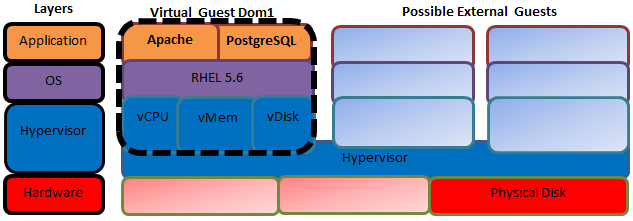
\includegraphics[width=6in]{images/LayersVirtualWithDisk.png}
  \caption{By passing the performance data from the physical resource to the guest Dom1 machine, the guest can determine if the interference is from an external layer.} 
  \label{LayersAndResourcesDisk}
  \end{center}
\end{figure}

There is a case when this could erroneously tell us there is interference when there is not any interference.  So far we have only examined systems where the application is running at 100\% of possible throughput.  One reason virtualization is successful is that not all guests run at full capacity at all times.  In a theoretically perfect virtualization, a physical resource $R$ would be divided between $n$ guests, and each guest would use $1/n$ of resource $R$ at all time.  For example, if a physical disk could handle a throughput rate of 400 reads per second, and 4 virtual machines each requested data at a rate of 100 reads per second. In this case, our method may inaccurately report 75\% interference.  

Since the guest has previously calculated the read wait time through the hypervisor $AvgRdWait$, we can use that information to determine if the guest is degraded due to interference from external systems.  When external systems are exceeding the I/O throughput, the $AvgRdWait$ time will increase significantly.  We can calculate the interference by using the average wait time (without interference) and the average wait time when run with additional external domains.  Since we are trying to determine if the hypervisor layer is the root cause, we need to use the information from the view of the hypervisor.

\begin{equation}
	Interference_{ARW} = \frac{AvgRdWait_{Current} - AvgRdWait_{Overhead}}{AvgRdWait_{Current}} 
\end{equation}

If both of the calculated interference results are positive then we can assume that the hypervisor is waiting for I/O, and there is something in the external layer that is the guest domain is not generating all of the I/O throughput.
Only when both of these values increase, can we accurately determine there is external interference.
We conclude that the interference from I/O reads is the lower of these two values.

\subsection{Hypervisor Interference}
Another option we explored was not consistent between workloads and system architectures.  The idea is to calculate the $Overhead_V$ again during production when calculating interference.  Instead of only using one guest we can calculate the total time spent waiting in all guests, and compare that to the hypervisor.  We call this calculation the $Overhead_{VALL}$ Since for one guest the time in that guest was always greater than the time in the hypervisor, we assume that the total time for all guests would increase.   The problem was that for some tests the hypervisor would generate extra reads and take more time than the guests.  We believe that the $Overhead_{VALL}$ may be a useful statistic for other resources.

\subsection{I/O Read Example Method}
First, the guest machine needs to calculate the $Overhead_V$ and save the $AvgRdWait_H$ for later reference.  When the guest machine is put into production, it can calculate the interference when requested from a user space tool.  Both the guest virtual machine and hypervisor can calculate the resource statistics according to algorithm in Figure \ref{alg1} when requested.  It is important that they collect $pre$ and $post$ statistics concurrently.  Then the hypervisor can return the $AvgRdWait$ and the $reads/s$ back to the guest.  Then the guest VM can calculate $Interference_{RPS}$ and $Interference_{ARW}$ as described previously.  The guest can report interference as the least of the two calculated interference measurements.

\begin{figure}[h]
\begin{algorithmic}[H]
 \STATE $Interference_{EXT} \gets 0$
 \IF{$Interference_{RPS} > 0$ \AND $Interference_{ARW} > 0$ } 
 	\STATE $Interference_{EXT} \gets FLOOR(Interference_{RPS}, Interference_{ARW})$  
 \ENDIF
\end{algorithmic}
\label{alg2}
\caption{User tool for guest domain to calculate external read I/O interference.}
\end{figure}

The user space tool \emph{iostat} reads disk performance counters in /proc/diskstats and will report transfers, bytes read, and bytes written per second.  If an application was experiencing I/O performance problems this would be a tool an administrator or application developer may monitor.  Without knowing the interference this could be misleading as to the root cause of the problem.  The following example shows a possible output from the perspective of the running guest when experiencing I/O interference from external guest machines.

\begin{figure}[h]
\begin{Verbatim}
Device:  tps    kB_read/s    kB_wrtn/s
sda   577.20     41388.00    148073.00
  I/O interference 22.4%     
\end{Verbatim}
\label{fig:iostat}
\caption{Example:  Possible \emph{iostat} output in a virtual guest experiencing external interference.  This is similar to the new \emph{steal time} for the CPU resource.}
\end{figure}

\subsection{Other Considerations}
There are three other issues that need to be considered with this type of method.  First, we examine the methods of passing information between the guests and hypervisor.  Second, we see if there are any performance issues with the method we describe.  Finally, we look at security concerns since passing information about external machines may reduce the security guarantees when a system is virtualized.

Most virtualization platforms have a message passing API native to the system.  Usually this is to automatically configure the guest domain when it is provisioned or when changes are needed.  For Xen Server, this is done through the Xenbus and Xenstore.  VMware guest tools has a guest API (vmware-tools-guestlib package), and even has a setting to pass host (hypervisor) resource counter data to the guest \cite{vmwarepubs}.  However, this is disabled by default and security tuning documents encourage explicitly setting it off for security reasons. If there were not any native mechanism to pass data between the guest and the host system, we could still use some message passing over TCP/IP such as SOAP or Rest service with HTTP.
%https://www.vmware.com/support/developer/guest-sdk/guest_sdk_40.pdf

There is some performance overhead with this additional data collection, as with any method that attempts to measure performance.  We do not want a tool to negatively impact the performance, or report degradation from the tool itself.  For I/O performance issues we believe that our method will not have a measurable impact.  For a system that is waiting on I/O from disk, it should have CPU cycles available for data processing.  Both the guest and the hypervisor need to read in memory kernel data twice.  Each layer needs to compute the difference of the two statistics after they are collected.  The hypervisor needs to pass the data to the guest VM, and then the guest needs to calculate the interference.  There are several tools in Windows and Linux that perform similar to this now (other than passing information), and are widely accepted.

Obviously, security is a major concern for a virtual machine that may be running concurrently with untrusted external systems.  The more information an attacker can gain about the system, the better chance that a vulnerability can be found.  There is similar precedence for sending this type of data in a standard kernel.  Currently (by default) all users can see the sum of the I/O and CPU processes.  The OS kernel has the responsibility to provide protection, yet it provides access to global data about the system.  This is the same type of data where we want to know how our virtual machine is effected by other virtual machines.  An attacker may be able to gain knowledge about the run state of external machines, and possibly execute some covert channel attacks.  It may be beneficial to limit the guest to only requesting data from the hypervisor at known time intervals.  More research would be needed to see what types of vulnerabilities would be possible, and what types of controls could be added to reduce the risk of an exploit.  

